%==============================================================================
% Figure: E8 Optimal Sphere Packing Visualization
% Source: Ch04 (E8 Lattice Theory)
% Framework: M (Mathematical) | Type: Geometric diagram
% Date: 2025-10-21
%==============================================================================

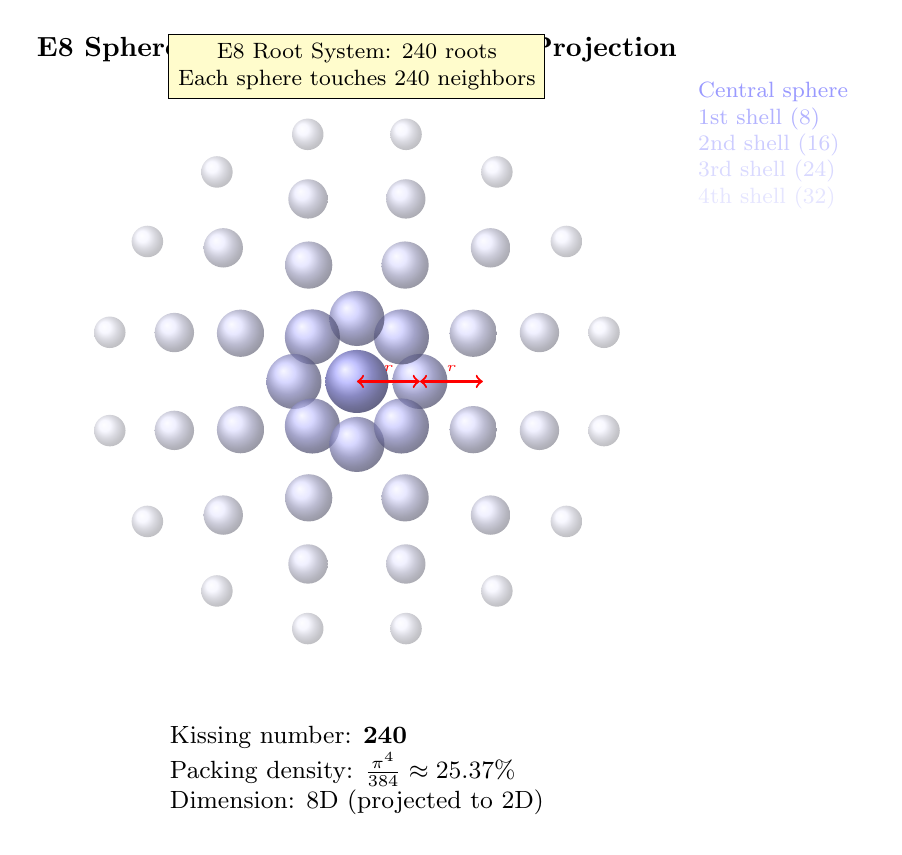
\begin{tikzpicture}[scale=1.0]
  % Title
  \node[anchor=north] at (0,4.5) {\textbf{E8 Sphere Packing: Coxeter Plane Projection}};

  % Central sphere
  \shade[ball color=blue!40!white, opacity=0.8] (0,0) circle (0.4);

  % Inner ring: 8 nearest neighbors (octonion directions)
  \foreach \angle in {0,45,90,135,180,225,270,315} {
    \shade[ball color=blue!30!white, opacity=0.7]
      ({0.8*cos(\angle)}, {0.8*sin(\angle)}) circle (0.35);
  }

  % Second ring: 16 neighbors
  \foreach \angle in {22.5,67.5,...,337.5} {
    \shade[ball color=blue!20!white, opacity=0.6]
      ({1.6*cos(\angle)}, {1.6*sin(\angle)}) circle (0.3);
  }

  % Third ring: 24 neighbors (partial, showing projection)
  \foreach \angle in {15,45,75,...,345} {
    \shade[ball color=blue!15!white, opacity=0.5]
      ({2.4*cos(\angle)}, {2.4*sin(\angle)}) circle (0.25);
  }

  % Outer ring: 32 neighbors (partial projection)
  \foreach \angle in {11.25,33.75,56.25,...,348.75} {
    \shade[ball color=blue!10!white, opacity=0.4]
      ({3.2*cos(\angle)}, {3.2*sin(\angle)}) circle (0.2);
  }

  % Annotations
  \node[anchor=north, font=\small] at (0,-4.2) {
    \begin{tabular}{l}
      Kissing number: \textbf{240} \\
      Packing density: $\frac{\pi^4}{384} \approx 25.37\%$ \\
      Dimension: 8D (projected to 2D)
    \end{tabular}
  };

  % Distance markers
  \draw[<->, thick, red] (0,0) -- (0.8,0) node[midway, above] {\tiny $r$};
  \draw[<->, thick, red] (0.8,0) -- (1.6,0) node[midway, above] {\tiny $r$};

  % Legend
  \node[anchor=west, font=\footnotesize] at (4,3) {
    \begin{tabular}{l}
      \textcolor{blue!40}{Central sphere} \\
      \textcolor{blue!30}{1st shell (8)} \\
      \textcolor{blue!20}{2nd shell (16)} \\
      \textcolor{blue!15}{3rd shell (24)} \\
      \textcolor{blue!10}{4th shell (32)}
    \end{tabular}
  };

  % E8 lattice annotation
  \node[draw, rectangle, fill=yellow!20, font=\footnotesize, align=center] at (0,4) {
    E8 Root System: 240 roots \\
    Each sphere touches 240 neighbors
  };

\end{tikzpicture}

% Usage: %==============================================================================
% Figure: E8 Optimal Sphere Packing Visualization
% Source: Ch04 (E8 Lattice Theory)
% Framework: M (Mathematical) | Type: Geometric diagram
% Date: 2025-10-21
%==============================================================================

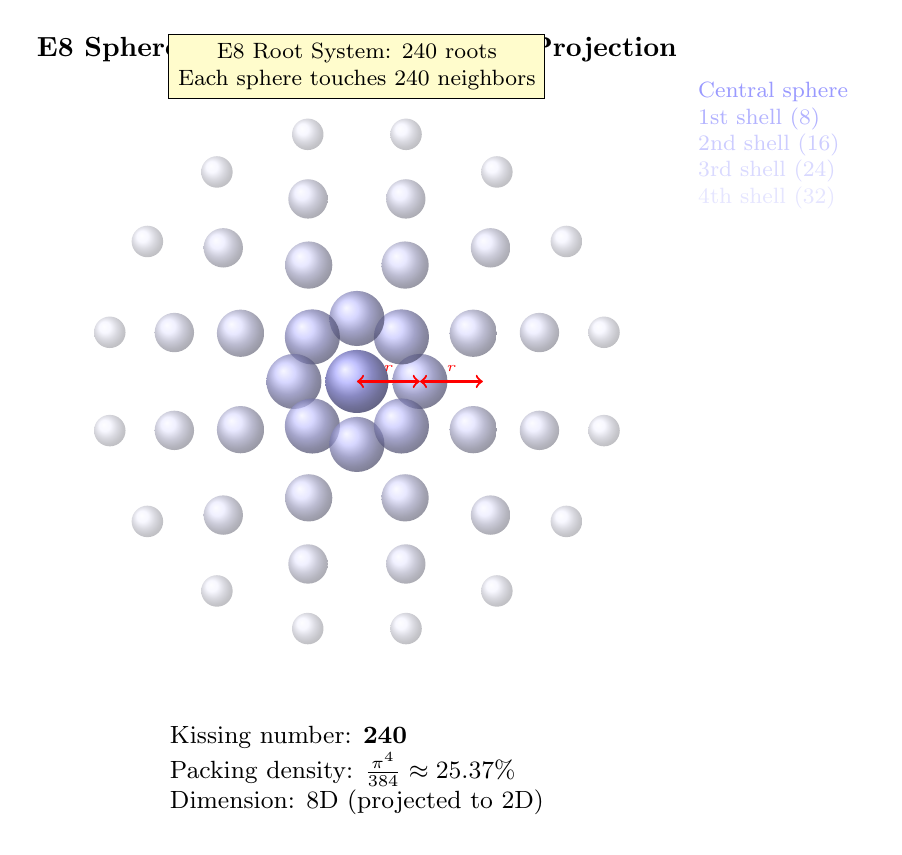
\begin{tikzpicture}[scale=1.0]
  % Title
  \node[anchor=north] at (0,4.5) {\textbf{E8 Sphere Packing: Coxeter Plane Projection}};

  % Central sphere
  \shade[ball color=blue!40!white, opacity=0.8] (0,0) circle (0.4);

  % Inner ring: 8 nearest neighbors (octonion directions)
  \foreach \angle in {0,45,90,135,180,225,270,315} {
    \shade[ball color=blue!30!white, opacity=0.7]
      ({0.8*cos(\angle)}, {0.8*sin(\angle)}) circle (0.35);
  }

  % Second ring: 16 neighbors
  \foreach \angle in {22.5,67.5,...,337.5} {
    \shade[ball color=blue!20!white, opacity=0.6]
      ({1.6*cos(\angle)}, {1.6*sin(\angle)}) circle (0.3);
  }

  % Third ring: 24 neighbors (partial, showing projection)
  \foreach \angle in {15,45,75,...,345} {
    \shade[ball color=blue!15!white, opacity=0.5]
      ({2.4*cos(\angle)}, {2.4*sin(\angle)}) circle (0.25);
  }

  % Outer ring: 32 neighbors (partial projection)
  \foreach \angle in {11.25,33.75,56.25,...,348.75} {
    \shade[ball color=blue!10!white, opacity=0.4]
      ({3.2*cos(\angle)}, {3.2*sin(\angle)}) circle (0.2);
  }

  % Annotations
  \node[anchor=north, font=\small] at (0,-4.2) {
    \begin{tabular}{l}
      Kissing number: \textbf{240} \\
      Packing density: $\frac{\pi^4}{384} \approx 25.37\%$ \\
      Dimension: 8D (projected to 2D)
    \end{tabular}
  };

  % Distance markers
  \draw[<->, thick, red] (0,0) -- (0.8,0) node[midway, above] {\tiny $r$};
  \draw[<->, thick, red] (0.8,0) -- (1.6,0) node[midway, above] {\tiny $r$};

  % Legend
  \node[anchor=west, font=\footnotesize] at (4,3) {
    \begin{tabular}{l}
      \textcolor{blue!40}{Central sphere} \\
      \textcolor{blue!30}{1st shell (8)} \\
      \textcolor{blue!20}{2nd shell (16)} \\
      \textcolor{blue!15}{3rd shell (24)} \\
      \textcolor{blue!10}{4th shell (32)}
    \end{tabular}
  };

  % E8 lattice annotation
  \node[draw, rectangle, fill=yellow!20, font=\footnotesize, align=center] at (0,4) {
    E8 Root System: 240 roots \\
    Each sphere touches 240 neighbors
  };

\end{tikzpicture}

% Usage: %==============================================================================
% Figure: E8 Optimal Sphere Packing Visualization
% Source: Ch04 (E8 Lattice Theory)
% Framework: M (Mathematical) | Type: Geometric diagram
% Date: 2025-10-21
%==============================================================================

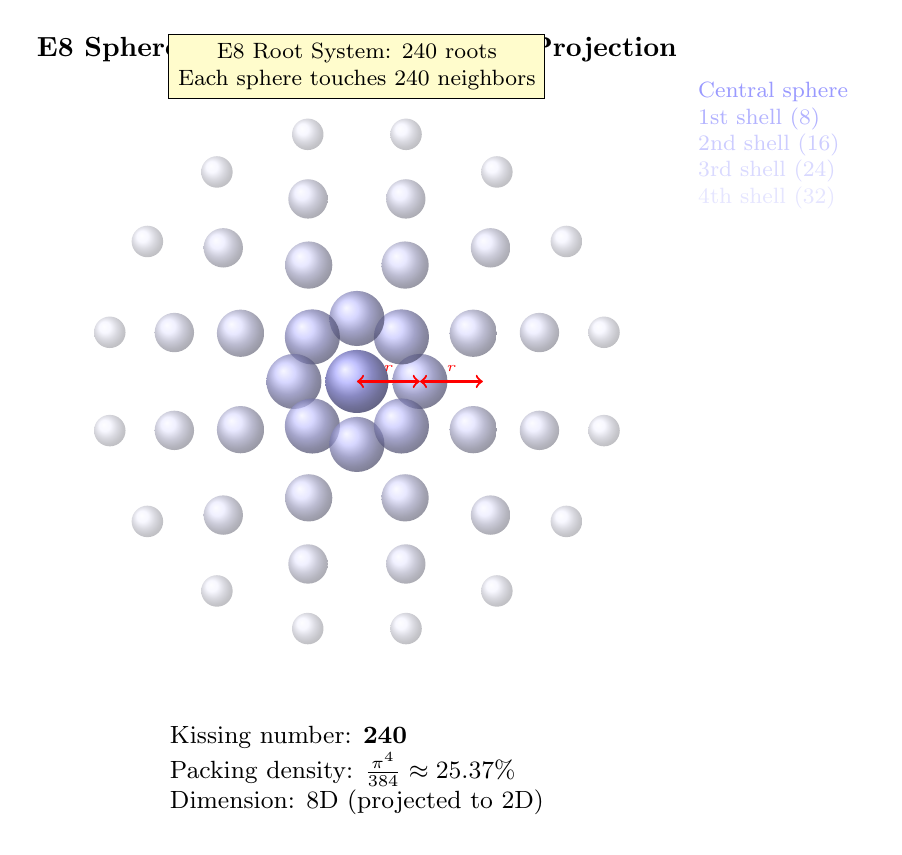
\begin{tikzpicture}[scale=1.0]
  % Title
  \node[anchor=north] at (0,4.5) {\textbf{E8 Sphere Packing: Coxeter Plane Projection}};

  % Central sphere
  \shade[ball color=blue!40!white, opacity=0.8] (0,0) circle (0.4);

  % Inner ring: 8 nearest neighbors (octonion directions)
  \foreach \angle in {0,45,90,135,180,225,270,315} {
    \shade[ball color=blue!30!white, opacity=0.7]
      ({0.8*cos(\angle)}, {0.8*sin(\angle)}) circle (0.35);
  }

  % Second ring: 16 neighbors
  \foreach \angle in {22.5,67.5,...,337.5} {
    \shade[ball color=blue!20!white, opacity=0.6]
      ({1.6*cos(\angle)}, {1.6*sin(\angle)}) circle (0.3);
  }

  % Third ring: 24 neighbors (partial, showing projection)
  \foreach \angle in {15,45,75,...,345} {
    \shade[ball color=blue!15!white, opacity=0.5]
      ({2.4*cos(\angle)}, {2.4*sin(\angle)}) circle (0.25);
  }

  % Outer ring: 32 neighbors (partial projection)
  \foreach \angle in {11.25,33.75,56.25,...,348.75} {
    \shade[ball color=blue!10!white, opacity=0.4]
      ({3.2*cos(\angle)}, {3.2*sin(\angle)}) circle (0.2);
  }

  % Annotations
  \node[anchor=north, font=\small] at (0,-4.2) {
    \begin{tabular}{l}
      Kissing number: \textbf{240} \\
      Packing density: $\frac{\pi^4}{384} \approx 25.37\%$ \\
      Dimension: 8D (projected to 2D)
    \end{tabular}
  };

  % Distance markers
  \draw[<->, thick, red] (0,0) -- (0.8,0) node[midway, above] {\tiny $r$};
  \draw[<->, thick, red] (0.8,0) -- (1.6,0) node[midway, above] {\tiny $r$};

  % Legend
  \node[anchor=west, font=\footnotesize] at (4,3) {
    \begin{tabular}{l}
      \textcolor{blue!40}{Central sphere} \\
      \textcolor{blue!30}{1st shell (8)} \\
      \textcolor{blue!20}{2nd shell (16)} \\
      \textcolor{blue!15}{3rd shell (24)} \\
      \textcolor{blue!10}{4th shell (32)}
    \end{tabular}
  };

  % E8 lattice annotation
  \node[draw, rectangle, fill=yellow!20, font=\footnotesize, align=center] at (0,4) {
    E8 Root System: 240 roots \\
    Each sphere touches 240 neighbors
  };

\end{tikzpicture}

% Usage: %==============================================================================
% Figure: E8 Optimal Sphere Packing Visualization
% Source: Ch04 (E8 Lattice Theory)
% Framework: M (Mathematical) | Type: Geometric diagram
% Date: 2025-10-21
%==============================================================================

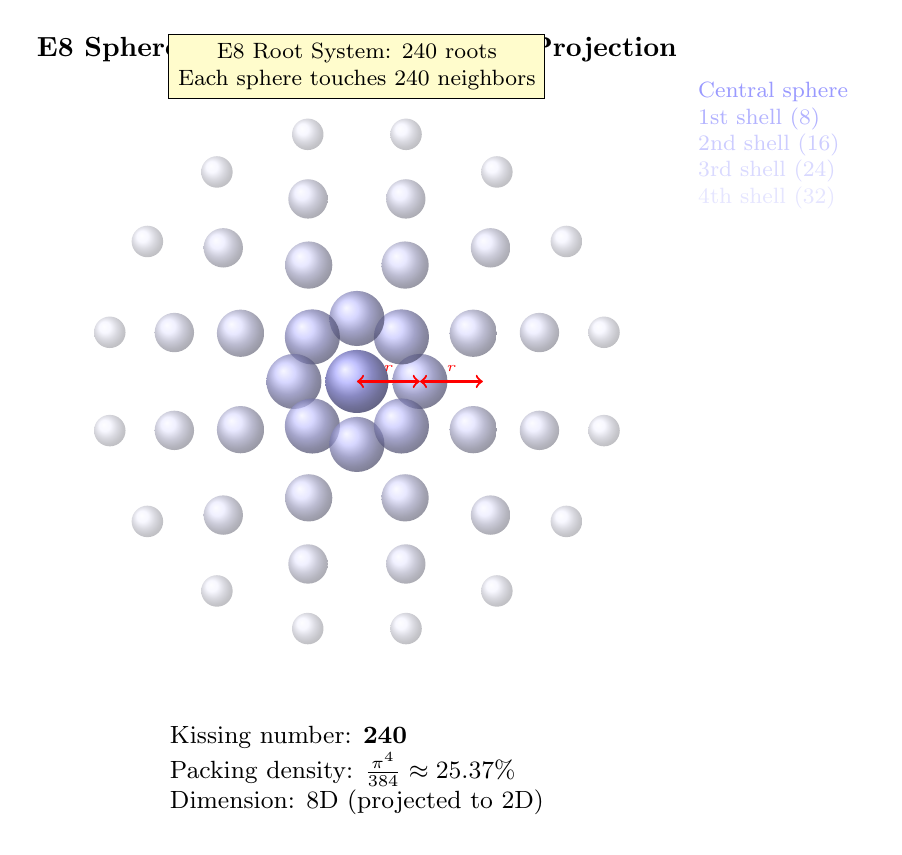
\begin{tikzpicture}[scale=1.0]
  % Title
  \node[anchor=north] at (0,4.5) {\textbf{E8 Sphere Packing: Coxeter Plane Projection}};

  % Central sphere
  \shade[ball color=blue!40!white, opacity=0.8] (0,0) circle (0.4);

  % Inner ring: 8 nearest neighbors (octonion directions)
  \foreach \angle in {0,45,90,135,180,225,270,315} {
    \shade[ball color=blue!30!white, opacity=0.7]
      ({0.8*cos(\angle)}, {0.8*sin(\angle)}) circle (0.35);
  }

  % Second ring: 16 neighbors
  \foreach \angle in {22.5,67.5,...,337.5} {
    \shade[ball color=blue!20!white, opacity=0.6]
      ({1.6*cos(\angle)}, {1.6*sin(\angle)}) circle (0.3);
  }

  % Third ring: 24 neighbors (partial, showing projection)
  \foreach \angle in {15,45,75,...,345} {
    \shade[ball color=blue!15!white, opacity=0.5]
      ({2.4*cos(\angle)}, {2.4*sin(\angle)}) circle (0.25);
  }

  % Outer ring: 32 neighbors (partial projection)
  \foreach \angle in {11.25,33.75,56.25,...,348.75} {
    \shade[ball color=blue!10!white, opacity=0.4]
      ({3.2*cos(\angle)}, {3.2*sin(\angle)}) circle (0.2);
  }

  % Annotations
  \node[anchor=north, font=\small] at (0,-4.2) {
    \begin{tabular}{l}
      Kissing number: \textbf{240} \\
      Packing density: $\frac{\pi^4}{384} \approx 25.37\%$ \\
      Dimension: 8D (projected to 2D)
    \end{tabular}
  };

  % Distance markers
  \draw[<->, thick, red] (0,0) -- (0.8,0) node[midway, above] {\tiny $r$};
  \draw[<->, thick, red] (0.8,0) -- (1.6,0) node[midway, above] {\tiny $r$};

  % Legend
  \node[anchor=west, font=\footnotesize] at (4,3) {
    \begin{tabular}{l}
      \textcolor{blue!40}{Central sphere} \\
      \textcolor{blue!30}{1st shell (8)} \\
      \textcolor{blue!20}{2nd shell (16)} \\
      \textcolor{blue!15}{3rd shell (24)} \\
      \textcolor{blue!10}{4th shell (32)}
    \end{tabular}
  };

  % E8 lattice annotation
  \node[draw, rectangle, fill=yellow!20, font=\footnotesize, align=center] at (0,4) {
    E8 Root System: 240 roots \\
    Each sphere touches 240 neighbors
  };

\end{tikzpicture}

% Usage: \input{modules/figures/fig_e8_sphere_packing.tex}
% Notes: This is a 2D Coxeter plane projection of the 8D E8 lattice sphere packing.
%        The full 240-sphere kissing configuration exists in 8 dimensions.
%==============================================================================

% Notes: This is a 2D Coxeter plane projection of the 8D E8 lattice sphere packing.
%        The full 240-sphere kissing configuration exists in 8 dimensions.
%==============================================================================

% Notes: This is a 2D Coxeter plane projection of the 8D E8 lattice sphere packing.
%        The full 240-sphere kissing configuration exists in 8 dimensions.
%==============================================================================

% Notes: This is a 2D Coxeter plane projection of the 8D E8 lattice sphere packing.
%        The full 240-sphere kissing configuration exists in 8 dimensions.
%==============================================================================
